\question{3}{5} The following shows a sequence of figures formed by sticks. The 1st figure has $4$ sticks. The 2nd figure has $12$ sticks. The 3rd figure has $24$ sticks. The 4th figure has $40$ sticks, and so on.

\par\vspace{0.5em}
\noindent\hspace*{2em}%
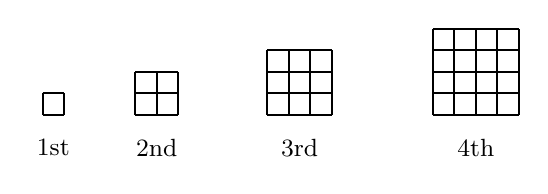
\begin{tikzpicture}[scale=0.42,baseline=-0.8ex,every node/.style={font=\small}]
  \foreach \f/\x/\n in {1/0/1, 2/2.8/2, 3/6.8/3, 4/11.8/4} {
    \foreach \i in {0,...,\n} {
      \draw[line width=0.7pt] (\x+\i*0.65,0) -- (\x+\i*0.65,\n*0.65);
    }
    \foreach \j in {0,...,\n} {
      \draw[line width=0.7pt] (\x,\j*0.65) -- (\x+\n*0.65,\j*0.65);
    }
    \ifnum\f=1 \def\flabel{1st}\fi
    \ifnum\f=2 \def\flabel{2nd}\fi
    \ifnum\f=3 \def\flabel{3rd}\fi
    \ifnum\f=4 \def\flabel{4th}\fi
    \node[below] at (\x+\n*0.65/2,-0.45) {\flabel};
  }
\end{tikzpicture}

\begin{subparts}
  \item According to the above pattern, guess the number of sticks used to form the 5th figure.
  \item A student claims that the number of sticks used to form the 6th figure is an odd number. Do you agree? Explain your answer.
\end{subparts}

\answerlines{16}
